\chapter{Circuit simulations for generating various waveform signals}
% Outline the simulation results based on the chosen approach in the previous chapter
The circuit simulations are run to validate the behaviour of the conceptual design of the Riemann Pump. The simulated output signal already identifies some fundamental ideas to understand the drawbacks and trade-offs of the designed circuit.\\
To investigate the theoretical concepts of chapter \ref{ch:design} the harmonic balance simulator is used.
The harmonic balance simulation is done with the design tool \gls{ab:ads}.
The benefit of the harmonic balance simulation is that the whole system is modelled in a steady state mode, so that no transients influences the results. \textit{"Harmonic balance is a frequency-domain analysis technique for simulating non linear circuits and systems[...]"}  ADS\_Harmonic\_Balance.pdf\\
In a first step the analog signal across the output impedance in the time domain is plotted to check whether a signal could be synthesized or not. 
After various signals could be synthesized, a short stability and energy consumption analysis is done.
The stability check is needed to validate that the circuit do not oscillate.
As well the circuits energy consumption has to be in a moderate range (\textit{which is the moderate range? mention it here?}) since it could be implemented in mobile devices.\\
    In the last step a simulation is run which makes the concept comparable to the realized circuit. 
   In this simulation the transistor dimensions are the same like the ones of the built demonstrator. However this simulation neglects losses due to the bonds and \gls{ab:msl}. This should give an insight to the behaviour of the constructed demonstrator.
   This is the first approach to see what could be expected from the built demonstrator.\\
   It is important to note that all simulations are done under ideal conditions and no losses due to the bonds and \gls{ab:msl} are taken into account. 
    The modelling of the designed circuit under real conditions, which include the exact calculation of all impedances of \gls{ab:msl} and bond wires would go beyond the scope of this thesis. Therefore a keep it small and simple approach is chosen to proof the concept.\\   

\section{Generating various analog signals with digital input control}
The generation of analog signals at the output of the designed \gls{ab:dac} is the goal of the concept. The designed Riemann Pump should be able to create various (arbitrary) waveform signals.
%To validate the feasibility of the presented concept, a digital input control code is required.
%To get this code an approximation by hand is done since no algorithm exists which can compute this.
Simulation in time domain is required to validate the correct generation of a signal. In fact of the linear approximation of current charging a capacitor this is the only way to verify the output signal. If this signal is confirmed to be as good as wanted, a frequency simulation can show the spurious free dynamic range or whatever which is important to mobile communication.
This digital to analog conversion is the crucial thing in the whole process.
Therefore this check of the conceptual idea of the schematic is essential.\\
To synthesize various analog signals in the time domain, the corresponding digital input code is needed. 
To get a certain analog signal at the output, a specific digital input code is needed, named here Riemann Code.
Due to the fact that no algorithm exists which computes the Riemann code, it is manually done by hand.\\ 
 The generation of the various analog output signals is based on the concept of chapter \ref{ch:design}. 
 The presented \gls{ab:dac} have a resolution of three bit and synthesizes signals with an \gls{ab:osr} of four. 
  The components are optimized with respect to the signal integrity. The dimensions of the used components are tuned while simulation to provide the desired output signal.
  In contrast to this optimized components, chapter \ref{ch:ProofOfConceptWithExistingComponents} deals with the simulation done with real dimensions of the demonstrator components. 
  This simulation is comparable to the realized demonstrator and shows what is expected for the measurements.
 
\subsection{Sine wave generation in the time domain}
As known from basic signal processing 
%[Oppenheim, MIT, Signals and Systems Lecture \textit{http://ocw.mit.edu/resources/res-6-007-signals-and-systems-spring-2011/lecture-notes/MITRES\_6\_007S11\_lec02.pdf}]
[REF.?] the sine wave for continuous time is the elementary signal and therefore synthesized first. 
For the generation of this sine wave a digital input code is required which will be converted to the analog output signal.\\
This digital input, called Riemann Code, is generated by hand with an approximation of a sine wave with eight different slopes at eight sampling points. 
The eight different slopes represents a three bit resolution of the \gls{ab:dac} while eight sampling points refer to the \gls{ab:osr}.\\
Figure \ref{fig:RiemannCodeGenerationSineWave} presents the sequence of slopes used to approximate a sine wave. 

\begin{figure}[htb!]
   \centering
   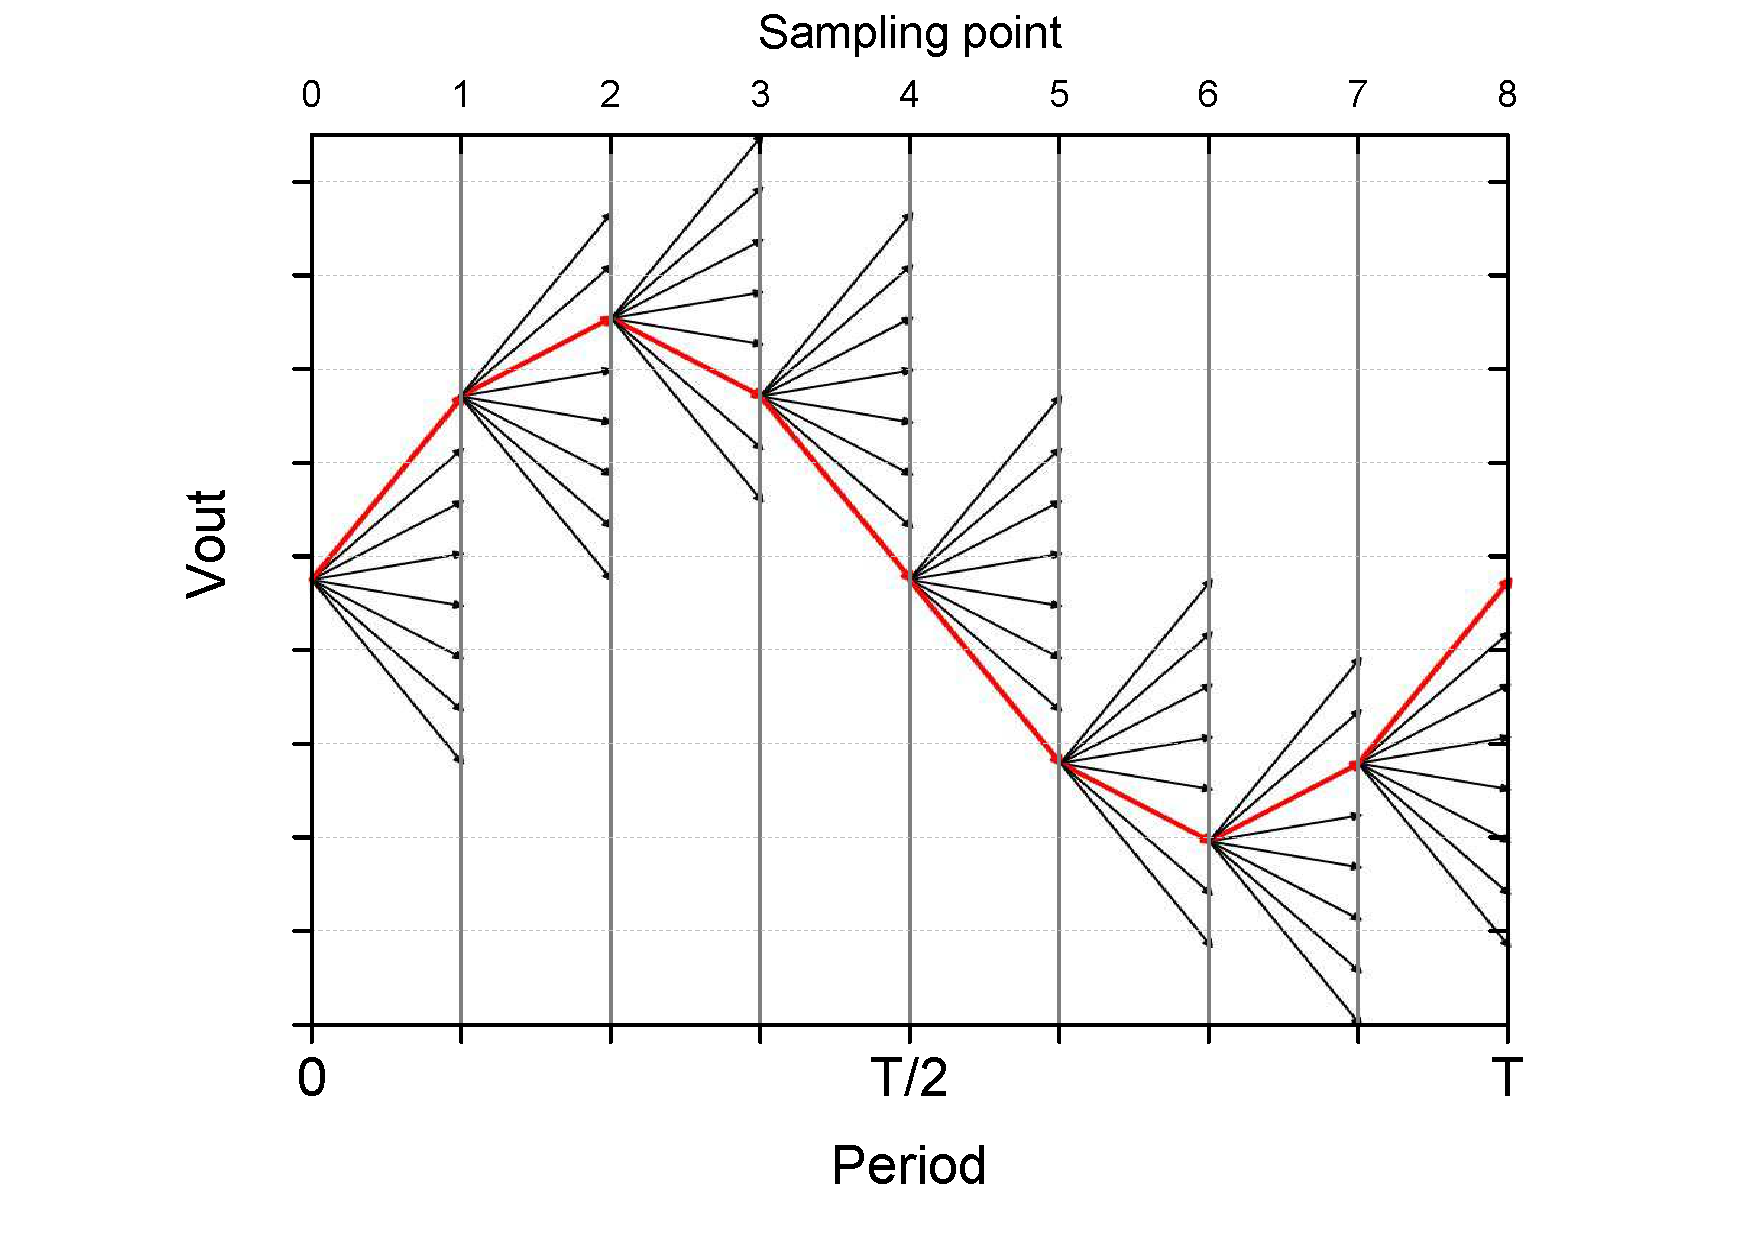
\includegraphics[width=0.75\textwidth]{RiemannCodeGeneration.pdf}
   \caption{One possible approximation of sine wave generation to get the Riemann Code}
   \label{fig:RiemannCodeGenerationSineWave}
\end{figure}

This sequence of slopes, referred to $i_0$ values, is:
\begin{equation}
 +7\hspace{.3cm} +3\hspace{.3cm} -3\hspace{.3cm} -7\hspace{.3cm} -7\hspace{.3cm} -3\hspace{.3cm} +3\hspace{.3cm} +7,
 \end{equation} which represents the following Riemann code:
\begin{equation}
000\hspace{.3cm} 010\hspace{.3cm} 101\hspace{.3cm} 111\hspace{.3cm} 111\hspace{.3cm} 101\hspace{.3cm} 010\hspace{.3cm} 000.
\end{equation}
\label{eq:RiemannCodeSineWave} 
   
 The Code consists of eight triplets where each triplet represent the three different switches and the half of the sampling points per period the \gls{ab:osr}.\\ 
This particular generated Riemann code was used to synthesize sine waves in the frequency range between \SI{500}{\MHz} and \SI{6}{\GHz}, as seen in Figure \ref{fig:7SignalsSameSlopeInOnePlot}.

\begin{figure}[htb!]
   %\centering
   \hspace{.8cm}
   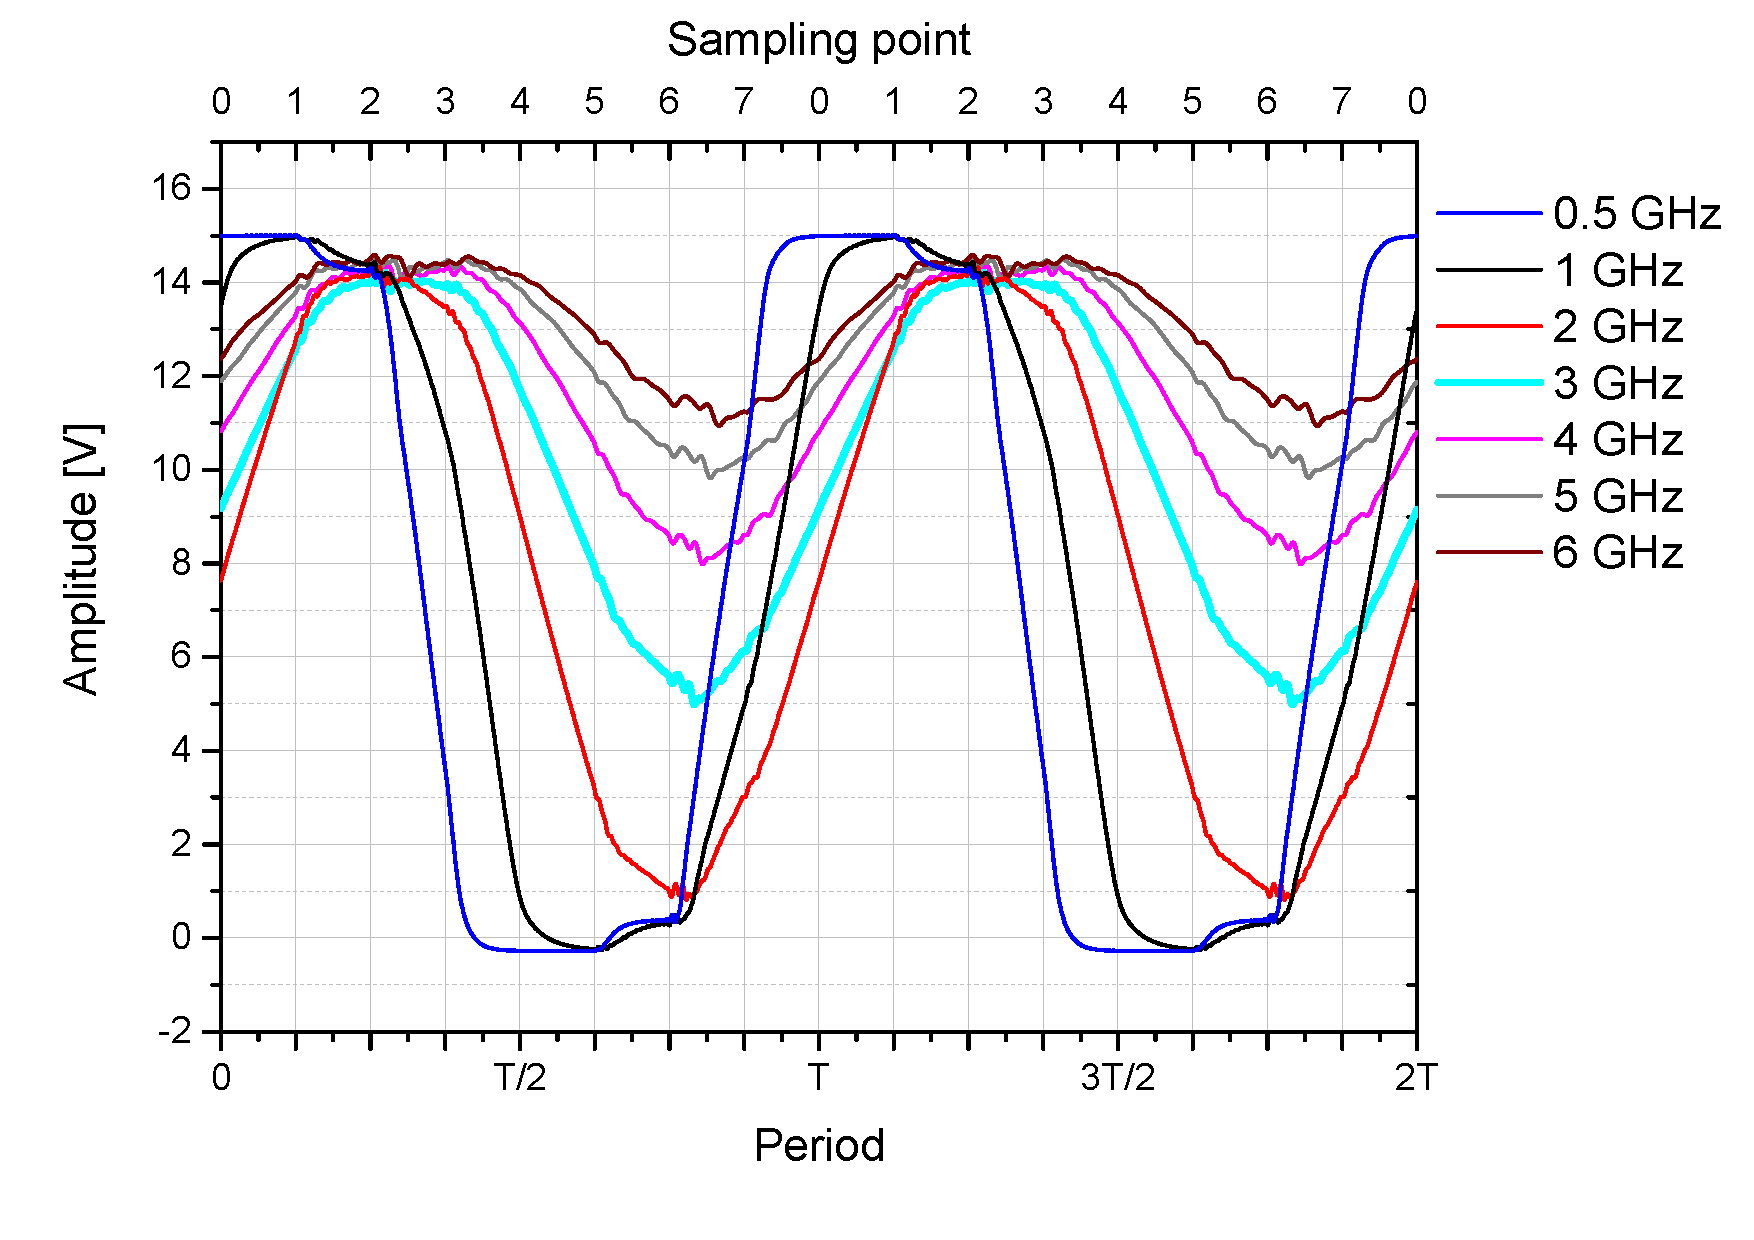
\includegraphics[width=0.75\textwidth]{Vout_sine_SigBWdifferent_SameSlope_73_PeriodT.pdf}
   \caption{Signals synthesized with demonstrated Riemann Code for the frequency range from \SI{500}{\MHz} to \SI{6}{\GHz} over two periods}
   \label{fig:7SignalsSameSlopeInOnePlot}
\end{figure}

The Figure \ref{fig:7SignalsSameSlopeInOnePlot} shows seven synthesized signals with the same input control code but with different sampling frequencies. 
The signals amplitudes are plotted over two periods in time domain.
Due to the different periods of sampling time the amplitude of each signal differs.
The maximum amplitude is the supply voltage of \SI{15}{\volt}. 
If this voltage is reached, the signal wave form is clipped and transforms the sine wave form into an rectangular.
The shape from most of the plotted functions fit fairly to the one of a theoretical sine wave.
But Figure \ref{fig:7SignalsSameSlopeInOnePlot} also highlights already some limitation of the designed circuit as the blue curve turns more into a rectangular signal form.\\

\begin{figure}[htb!]
   \centering
   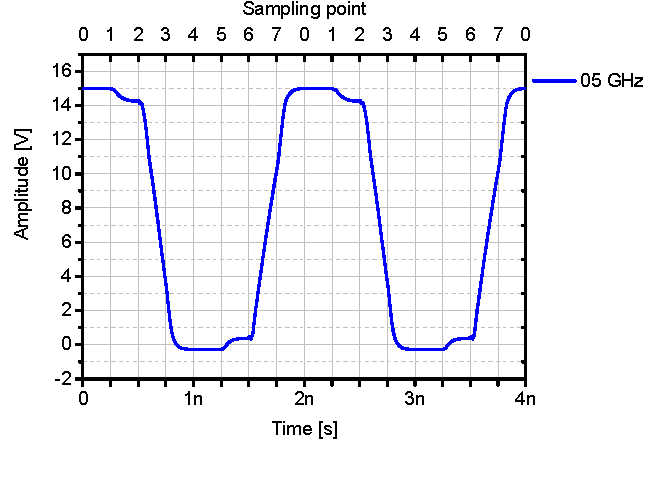
\includegraphics[width=0.75\textwidth]{Vout_sine_SigBW_05GHz_3bit_long.pdf}
   \caption{Synthesized sine wave for frequency of 0.5GHz}
   \label{fig:SineWave05GHz}
\end{figure}

The circuit designed in chapter \ref{ch:design} is optimized to cover the frequency range from \SI{1}{\GHz} to \SI{6}{\GHz} fairly well, if a voltage swing of nearly  two volts is still acceptable at \SI{6}{\GHz}.
If we go beneath a frequency of \SI{1}{\GHz} the desired shape of a sine wave is going to be rectangular due to the long sampling time refer to Figure \ref{fig:SineWave05GHz}.\\
The blue signal which should represent a sine wave with a signal frequency of \SI{500}{\MHz} is clipped and hence shows the behaviour of a rectangular signal.
 This undesired behaviour is induced from a fully charged output capacitance.
This is the lower bound on the frequency range for the signals.
Using the \gls{ab:osr} of four, we already get a sampling frequency of \SI{2}{GHz} at the lower bound.
For this reason the switches have to switch within \SI{0.5}{\nano \second} which increase the gate drive current which increase the power loss.
%This lower bound could be shifted to even lower frequencies if the dimensions are tuned to be smaller
The upper bound on the frequency range is the at least detectable voltage swing which could be amplified.
% to increase this upper bound the transistor dimension have to be bigger


%%% put in the limitation here or later in a seperate paragraph???

Figure \ref{fig:SineWaveSynthVsTheoretical} compares a theoretical sine wave signal (red) with the synthesized one (black) for a frequency of \SI{1}{\GHz}.
The synthesized signal is represented in Figure \ref{fig:7SignalsSameSlopeInOnePlot} as the black curve.
%, which within this scale already seems to turn into a rectangular signal form.
Setting up the right parameters, a good approximation of a sine wave can be performed.\\
In general the sine wave is of the form: 
\begin{equation}
	v(t)= V_{DC} + \widehat{v} \cdot sin( 2  \pi  f \cdot  t + \phi).
\end{equation}
The synthesized signal (black) in Figure \ref{fig:SineWaveSynthVsTheoretical} fits pretty good to the theoretical sine wave with an amplitude of $\widehat{v} = \SI{7.5}{\volt}$, a signal frequency of $f = \SI{1}{\giga \hertz}$, a phase shift of $\phi = \pi / 4$ and an DC offset of $V_{DC} = \SI{7.5}{\volt}$.

\begin{figure}[htb!]
   \centering
   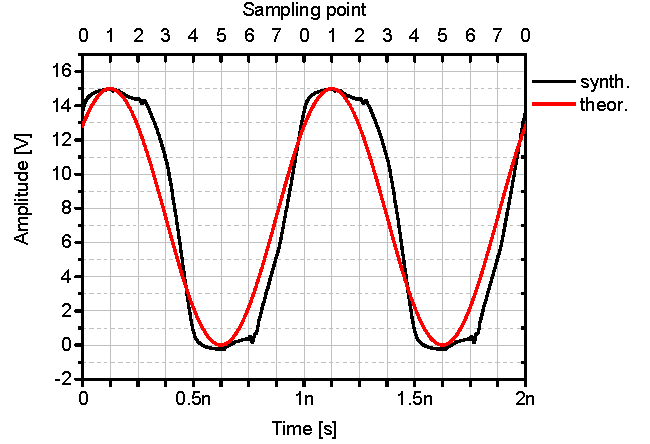
\includegraphics[width=0.75\textwidth]{Vout_SynthVsTheo.pdf}
   \caption{Synthesized sine wave with the theoretical sine wave}
   \label{fig:SineWaveSynthVsTheoretical}
\end{figure}

The fit seems to be very good but two distortions are visible in the peak and the valley of the synthesized signal.
($\rightarrow$Why are these two distortions?$\leftarrow$)
The fit is not perfect since the digital to analog conversion always introduce noise to the signal, refer to chapter \ref{ch:fundamentals} and the \gls{ab:sqnr}.\textbf{compare to the characteristic of DAC. Which SQNR is expected, which is achieved? $\rightarrow$ plot?} \\
The deviation of the synthesized signal from a theoretical sine wave is highlighted in Figure \ref{fig:SineCompare}.

\begin{figure}[htb!]
	\centering
  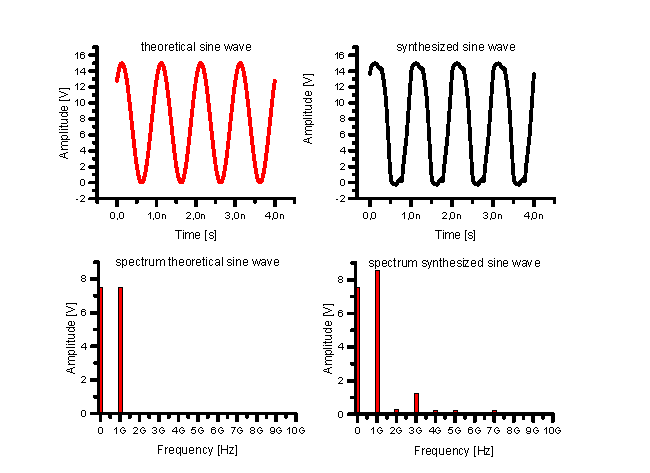
\includegraphics[width=1\textwidth]{SineCompare.pdf}
	\caption{Comparison between a theoretical and a synthesized sine wave with their spectrum}
	\label{fig:SineCompare}
\end{figure}

Here a sine wave is compared to the synthesized one with their corresponding spectra.
The spectra of signals are a lot easier to compare with respect to the accuracy in contrast to the time domain signal.
The spectrum of the signal points out how accurate the signal is synthesized compared to a perfectly shaped sine wave. 
Since the spectrum of a perfect sine wave only consists of a DC part and the harmonic frequency where it is swinging.\\
On the top left side the theoretical sine wave is plotted in red. Underneath of it the spectrum states a frequency portion for the direct component at \SI{0} {\GHz} and a fundamental frequency portion at \SI{1}{\GHz}.
This Fourier transformation represents the theoretic frequency portions of a clear sine wave. 
In comparison to this it seems that the synthesized signal on the top right side be a good approximation.
The spectrum on the bottom right side exhibits some distortion induced from the quantization process. 
Beside the direct component and the fundamental frequency component there are some other frequency portions which do not occur in the optimal sine wave spectrum.
This distortion are at maximal \SI{1}{\volt} in amplitude at a the third harmonic. The 2nd to 10th harmonic are at most a half of a volt. \\
\textit{The accuracy is very good. This can be verified by the signal to noise ratio -> explain, state the SNR}


As the sampling frequency can be changed to tune the signal frequency of the output signal it is also possible to change the input control sequence to manipulate the shape of the signal.
If the five possible Riemann Codes are applied to the circuit, the signal forms of Figure \ref{fig:SameSigBWDifSlope} would be generated.

\begin{figure}[htb!]
	\centering
  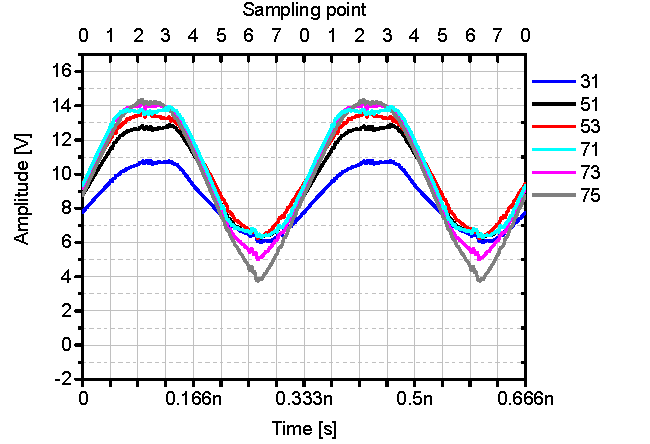
\includegraphics[width=1\textwidth]{Vout_7sine_SameSigBWdifferent_DifferentSlope.pdf}
	\caption{Signals with the same signal bandwidth but different input control}
	\label{fig:SameSigBWDifSlope}
\end{figure}

This plots the conversion of the different input signals over two periods for the signal frequency of \SI{3}{\GHz}.
The curves are named with 31, 51, 53, 73 and 75 which stands for the combination of the two slopes needed to approximate manually a sine wave.
The \gls{ab:osr} limits the number of different slopes to two, since otherwise it would increase the \gls{ab:osr} if we take, 753 and so on.
If the \gls{ab:osr} is increased the switching frequency is also increased and therefore the power consumption.
In addition to the power consumption problem, the components have a unity current gain frequency limit.
Figure \ref{fig:SameSigBWDifSlope} shows the range of the amplitude by applying different combination of slopes to approximate the sine wave signal.
Here are the five different slope combination plotted for a given signal frequency of \SI{3}{\GHz} and a \gls{ab:osr} of four.
The slope combination are limited to the resolution of the \gls{ab:dac}.
In fact of the three bit resolution only eight different slopes are available, for which four are positive and the counterparts are negative.
Therefore only a limited number of maximum six combination are existing to synthesize a sine wave form.
If the resolution have to be increased the whole circuit would become more complex and therefore the energy consumption would increase.
But also the signal integrity would be better, the accuracy better and the SQNR would be better.
To proof the concept a design is chosen to show the feasibility and in no way optimizing due to signal to noise ratio or to the energy consumption.

\subsection{rectified sine wave generation in the time domain}
Based on the same approximation principle of the signal in Figure \ref{fig:SineWaveCodeGeneration}, the Riemann Code for the rectified sine is generated. 
The chosen Riemann Code for the rectified sine is:
\begin{equation}
 000\hspace{.3cm} 010\hspace{.3cm} 101\hspace{.3cm} 111\hspace{.3cm} 000\hspace{.3cm} 010\hspace{.3cm} 101\hspace{.3cm} 111.
\end{equation}
\label{eq:RiemannCodeRectSine}

Using this code a rectified sine wave is synthesized by the designed circuit.
The generation of the rectified sine wave is the same as for the normal sine wave. 
This only shows a different signal which could be synthesized.






\subsection{triangular wave generation in the time domain}
This is a triangular wave.


\section{Stability analysis of the realised circuit}
The stability and energy consumption analysis helps to get an impression/ understanding of figures and numbers of the designed circuit. Although this two aspect are of an important role for the development of a high speed \gls{ab:dac} this analysis are not complete. The whole detailed analysis could not be investigated in this thesis due to complexity and time issues, what its meaning is not to belittle. For these aspects it is important to state that the designed circuit is in no way optimized with respect to those \\
The stability analysis is important to ensure that the circuit under test do not oscillate. 
 To check this, the complex impedance at specific points in the circuit is measured.
 If the real part of the impedance is positive for the whole frequency range of the simulation, it indicates in an easy way that the circuit does not oscillate.
This simulation is done within the ADS tool. 

\section{Energy consumption analysis of the realised circuit}
Due to the idea to use the presented topic for mobile communication it could be implemented in mobile devices, although this thesis only handles the device for the basestation. If it could be used in a mobile device the energy consumption is critical.\\
The energy consumption of the designed circuit in chapter \ref{ch:design} is simulated with \gls{ab:ads}.\\
 For the chips used for the demonstrator refer to the work of Stephan Maroldt who states, that the power consumption is:  divided into static and dynamic ones. The switching losses are greater than the static ones.
The losses are divided into dynamic losses of the switches and static losses.
% switch voltage for on/off state, switch time, static losses and dynamic losses.

\section{Proof of concept simulation with existing components}
\label{ch:ProofOfConceptWithExistingComponents}
This simulation is based on the measurements and the design of various chips from Stephan Maroldt.
This two bit resolution simulation is done to compare the demonstrators measurements with the simulation. \textbf{two-bit resolution, osr = 4, keep it small and simple, frequency higher, demonstrator, assembly, less complex} 
The three bit resolution DAC was too complex to realize in a first approach on a hybrid substrate. Therefore an easier approach was designed to validate the proof of concept.

\section{Evaluation of the simulation results for the Riemann Pump}
Nonetheless the number of signals which can be synthesized with this particular concept is increased with the possibility to change to another combination of slopes to approximate the signal.
All this calculation should be done with a signal processor and an algorithm.
With the variation of the slopes and the variation of the sampling time in theory it is possible to create every single signal with more or less good \gls{ab:sqnr}.
\\
When the component dimensions, like the switching transistors and load impedance, are fixed it is impossible to reach a bandwidth which goes from\gls{ab:dc} to \SI{6}{\GHz}.
The issue is that a small transistor dimension could synthesize signals to a very low signal frequency but will be unable to synthesize a signal at 6GHz due to the fact that the amplitude would be too small.
Hence the signal frequency bandwidth would be shifted to the smaller frequencies. 
If the \gls{ab:osr} is increased, the sampling time is decreased and therefore the signal quality is better because we have a more accurate synthesized signal. \\
If the transistor dimension is chosen to be bigger, the higher signal frequency could be synthesized with a decent voltage swing but the low signal frequencies would turn into a rectangular shape. 
This is the trade off between the shift of the bandwidth (shifting to even higher frequencies is possible but the bandwidth is nearly constant as long the output capacitance is constant too.) The trade off for the bandwidth shift to higher frequencies is, that with the signal frequency the switching frequency is increasing linearly (for an osr; eight times) and therefore the dynamic losses are increasing with this switching frequency.
By the way the transistor switching speed is determined by the dimension of the driver circuit, so if the switching speed is increased the gate driving current has to be increased to switch the transistors.

 The presented results show the theoretical feasibility of the approach.
 In a more enhanced project a MATLAB algorithm would compute this code by minimizing the deviation between a theoretical signal and the synthesized signal.
evaluate the simulation results, what is to expect in realisation. 
What is the expectation to the measurement?
